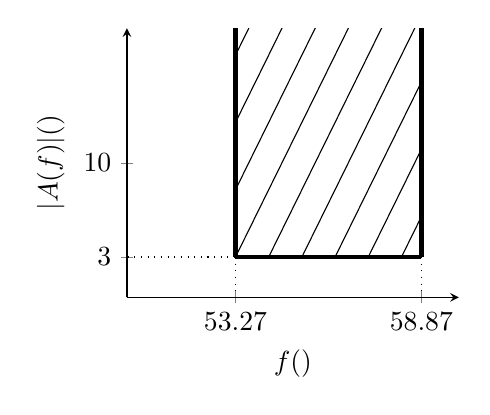
\begin{tikzpicture}
\begin{axis}[
    axis lines = left,
    xlabel = $f(\si{\kilo\hertz})$,
    ylabel = $|A(f)|(\si{\deci\bel})$,
    xmin = 50,
    xmax = 60,
    ymin = 0,
    ymax = 20,
    xtick = {0, 53.27, 58.87 },
    ytick = {3, 10 },
    height= 5cm
]
\addplot[
	domain=53.27:58.87,
	samples=10,
	color = black,
	ultra thick
] {3};
\addplot[domain=54.27:58.87,samples=10,color = black] {3+(x-54.27)*5};
\addplot[domain=55.27:58.87,samples=10,color = black] {3+(x-55.27)*5};
\addplot[domain=56.27:58.87,samples=10,color = black] {3+(x-56.27)*5};
\addplot[domain=57.27:58.87,samples=10,color = black] {3+(x-57.27)*5};
\addplot[domain=58.27:58.87,samples=10,color = black] {3+(x-58.27)*5};
\addplot[domain=53.27:58.87,samples=10,color = black] {3+(x-53.27)*5};
\addplot[domain=53.27:58.87,samples=10,color = black] {8+(x-53.27)*5};
\addplot[domain=53.27:58.87,samples=10,color = black] {13+(x-53.27)*5};
\addplot[domain=53.27:58.87,samples=10,color = black] {18+(x-53.27)*5};
\addplot[domain=53.27:58.87,samples=10,color = black] {23+(x-53.27)*5};
\addplot[domain=53.27:58.87,samples=10,color = black] {28+(x-53.27)*5};
\addplot[domain=53.27:58.87,samples=10,color = black] {33+(x-53.27)*5};
\addplot[domain=53.27:58.87,samples=10,color = black] {38+(x-53.27)*5};
\addplot[
	color=black,
	mark=none,
	ultra thick
]  coordinates {(53.27,3) (53.27,40) };
\addplot[
	color=black,
	mark=none,
	ultra thick
]  coordinates {(58.87,3) (58.87,40) };

\addplot[
	color=black,
	mark=none,
	dotted
]  coordinates {(53.27,3) (53.27,0) };
\addplot[
	color=black,
	mark=none,
	dotted
]  coordinates {(58.87,3) (58.87,0) };
\addplot[
	color=black,
	mark=none,
	dotted
]  coordinates {(0,3) (53.27,3) };

\end{axis}
\end{tikzpicture}